\documentclass[11pt]{article}
\usepackage[utf8]{inputenc}

%% Language and font encodings
\usepackage[english]{babel}
\usepackage[T1]{fontenc}
\usepackage[top=2cm,bottom=2cm,left=2cm,right=2cm,marginparwidth=1cm]{geometry}

%% Useful packages
\usepackage{amsmath}
\usepackage{amssymb}
\usepackage[shortlabels]{enumitem}
\usepackage{amsthm}
\usepackage{graphicx}
\usepackage{natbib}
\usepackage{setspace}
\usepackage[colorinlistoftodos]{todonotes}
\usepackage[colorlinks=true, allcolors=blue]{hyperref}
\DeclareMathOperator*{\argmax}{arg\,max}

%% Spacing 

\setlength{\parindent}{0pt}
\setlength{\parskip}{1em}

%% Remove spacing between list items

\setlist{nosep}


\usepackage[compact]{titlesec}
\titlespacing{\section}{0pt}{*-1}{*-1}
\titlespacing{\subsection}{0pt}{*0}{*0}
\titlespacing{\subsubsection}{0pt}{*0}{*0}

\usepackage{enumitem}
\title{\textbf{ECON 0200 | Example Exam} \\ Given: Monday, April 22}
\author{}
\date{}

\begin{document}
\maketitle
\vspace{-2cm}
Name: \raisebox{-1ex}{\rule{6.3cm}{1pt}}  \hfill Student ID: \raisebox{-1ex}{\rule{6.3cm}{1pt}}

This Final Exam will take 1 hour and 50 minutes. Exams are designed to both test your knowledge and challenge you to apply familiar concepts in new environments. Treat it as if you're trying to show me that you understand the material. Answer clearly and completely. 


\section*{Academic Conduct Code
}
The following academic conduct code is designed to protect the integrity of your work, not to make school feel overbearing. Print your name/initials beside the five academic honesty agreements before beginning. 


I pledge to my fellow students, the university and the instructor, that:

\raisebox{-1ex}{\rule{1.2cm}{1pt}} I will complete this MiniExam solely using my own work. 

\raisebox{-1ex}{\rule{1.2cm}{1pt}} I will not use any digital or hardcopy resources unless explicitly allowed by the instructor.

\raisebox{-1ex}{\rule{1.2cm}{1pt}} I will not communicate with others about the MiniExam in the room or remotely. 

\raisebox{-1ex}{\rule{1.2cm}{1pt}} I will not discuss the MiniExam with students who did not take the MiniExam at the same time.


\pagebreak

\subsection*{Game 1 (of 11). For the following game:
}
$$
\begin{array}{lccc}
    & & & (1-x) \ \ \ \ x\\
    & & & \text{L} \ \ \ \ \text{R}\\
    & &
    \begin{array}{r}
        y \ \ \text{U} \\
        (1-y) \ \ \text{D} \\
    \end{array} &
    \begin{array}{|c|c|}
        \hline
        9,4 & 13,3 \\
        \hline
        4,6 & 13,7 \\
        \hline
    \end{array}
\end{array}
$$


\begin{enumerate}[label=\alph*), start=1]
\item  Which outcomes are Pareto optimal (\textit{if none, write "none"})? \hfill \raisebox{-1ex}{\rule{4.2cm}{1pt}}

\end{enumerate}
\begin{enumerate}[label=\alph*), start=2]
\item  List all NE in pure strategies. \hfill \raisebox{-1ex}{\rule{4.2cm}{1pt}}

\end{enumerate}
\begin{enumerate}[label=\alph*), start=3]
\item  Is this game zero sum? \hfill \raisebox{-1ex}{\rule{4.2cm}{1pt}}

\end{enumerate}
\begin{enumerate}[label=\alph*), start=4]
\item  List all dominant strategies for this game (\textit{if none, write "none"}). \hfill \raisebox{-1ex}{\rule{4.2cm}{1pt}}

\end{enumerate}
\begin{enumerate}[label=\alph*), start=5]
\item  Plot both player’s best responses and all MSNE on the graph below.

\end{enumerate}

\begin{figure}[h!]
\centering
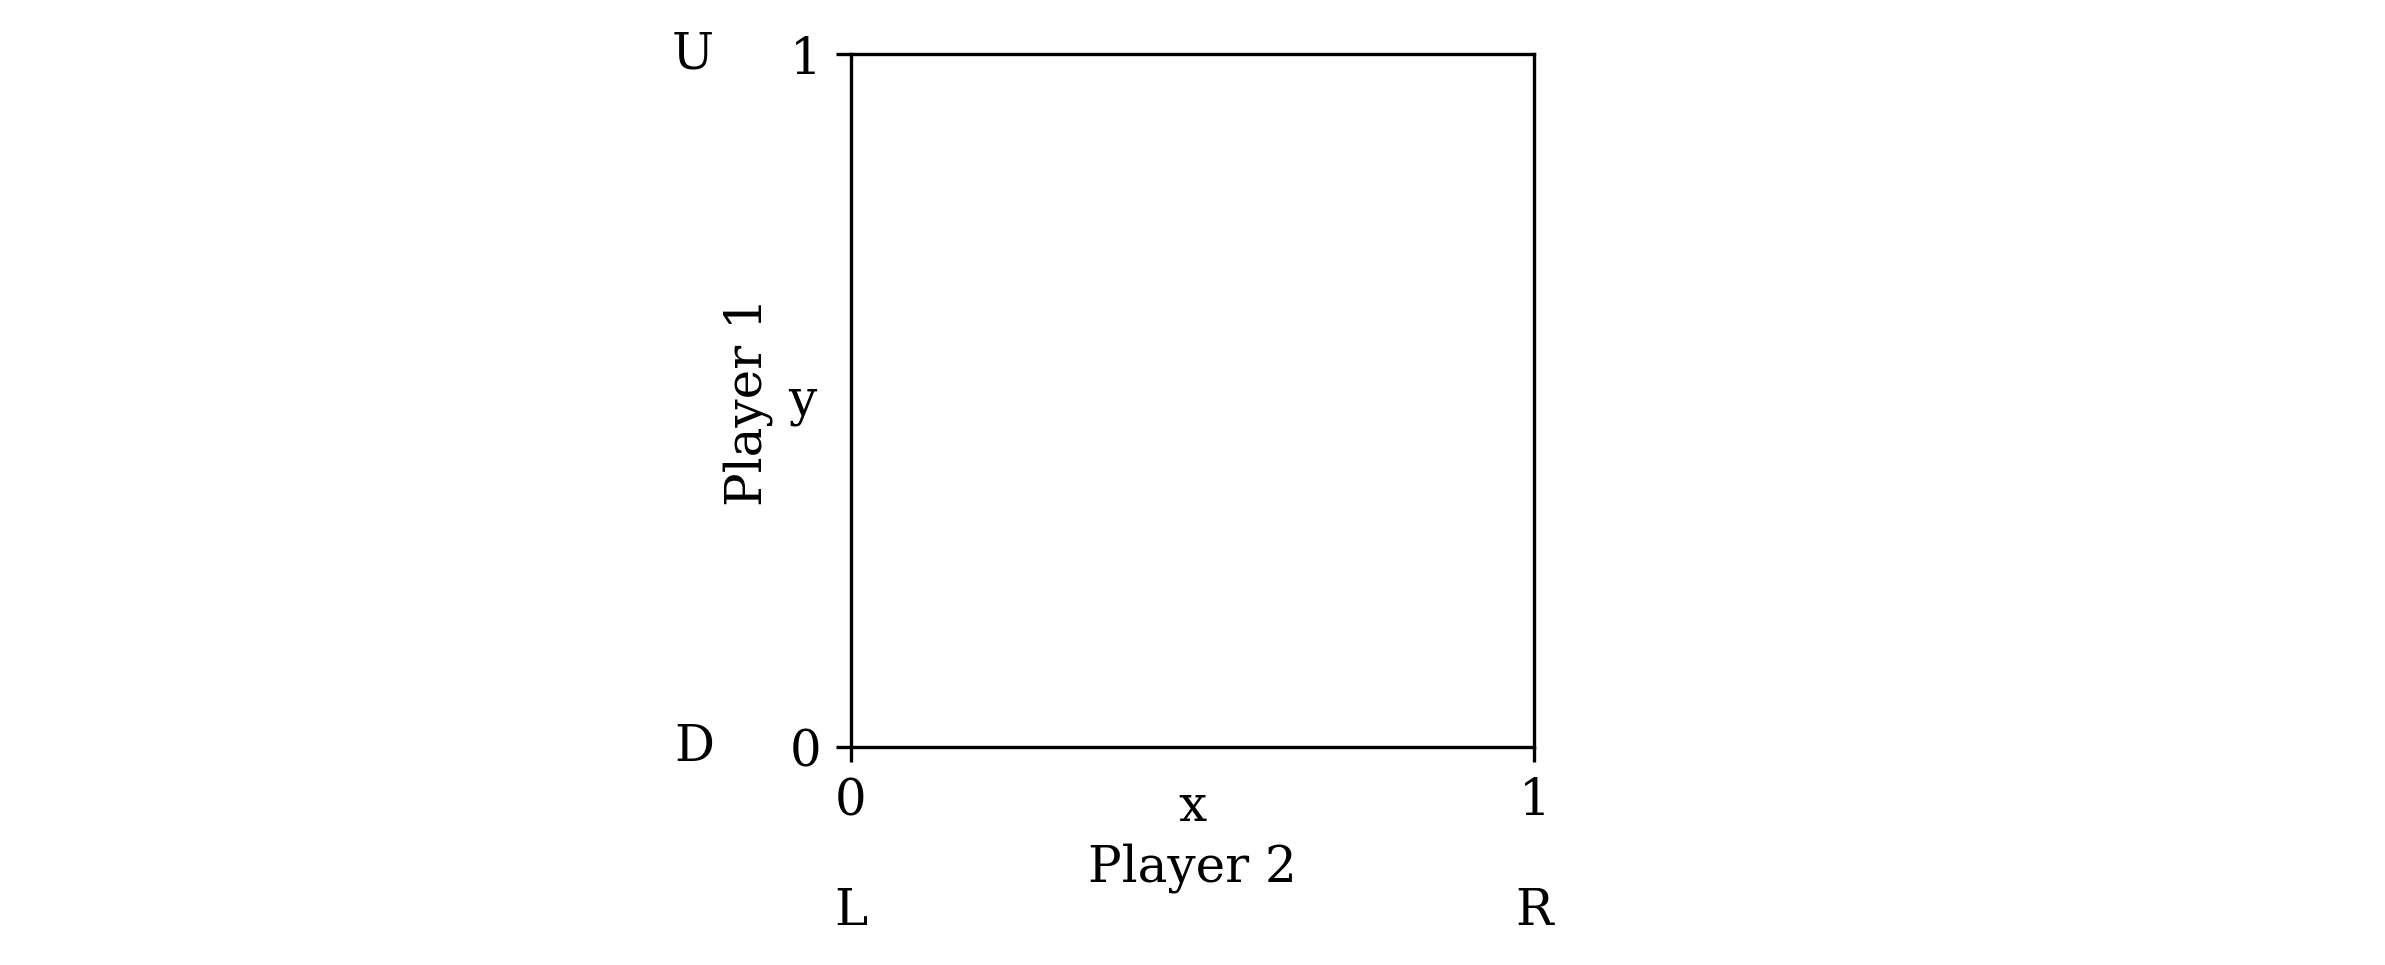
\includegraphics[width=\textwidth]{Images/mixed_strategy_graph.png}
\end{figure}

\pagebreak

\subsection*{Game 2 (of 11). Use Version 1 for a through e. Use Version 2 for f through l.
}
$$
\begin{array}{lcr}
\begin{array}{lccc}
    & & & \textbf{Version 1} \\
    & & & (1-x) \ \ \ \ x\\
    & & & \text{L} \ \ \ \ \text{R}\\
    & &
    \begin{array}{r}
        y \ \ \text{U} \\
        (1-y) \ \ \text{D} \\
    \end{array} &
    \begin{array}{|c|c|}
        \hline
        1,1 & 15,4 \\
        \hline
        4,15 & 7,7 \\
        \hline
    \end{array}
\end{array}
&
\begin{array}{lccc}
    & & & \textbf{Version 2} \\
    & & & (1-f) \ \ \ \ f\\
    & & & \text{A} \ \ \ \ \text{B}\\
    & &
    \begin{array}{r}
        \text{A} \\
        \text{B} \\
    \end{array} &
    \begin{array}{|c|c|}
        \hline
        1 & 15 \\
        \hline
        4 & 7 \\
        \hline
    \end{array}
\end{array}
\end{array}
$$


\begin{enumerate}[label=\alph*), start=1]
\item  Which outcomes are Pareto optimal (\textit{if none, write "none"})? \hfill \raisebox{-1ex}{\rule{4.2cm}{1pt}}

\end{enumerate}
\begin{enumerate}[label=\alph*), start=2]
\item  List all NE in pure strategies. \hfill \raisebox{-1ex}{\rule{4.2cm}{1pt}}

\end{enumerate}
\begin{enumerate}[label=\alph*), start=3]
\item  Is this game zero sum? \hfill \raisebox{-1ex}{\rule{4.2cm}{1pt}}

\end{enumerate}
\begin{enumerate}[label=\alph*), start=4]
\item  Plot both player’s best responses and all MSNE on the graph below.

\end{enumerate}


\begin{figure}[h!]
\centering
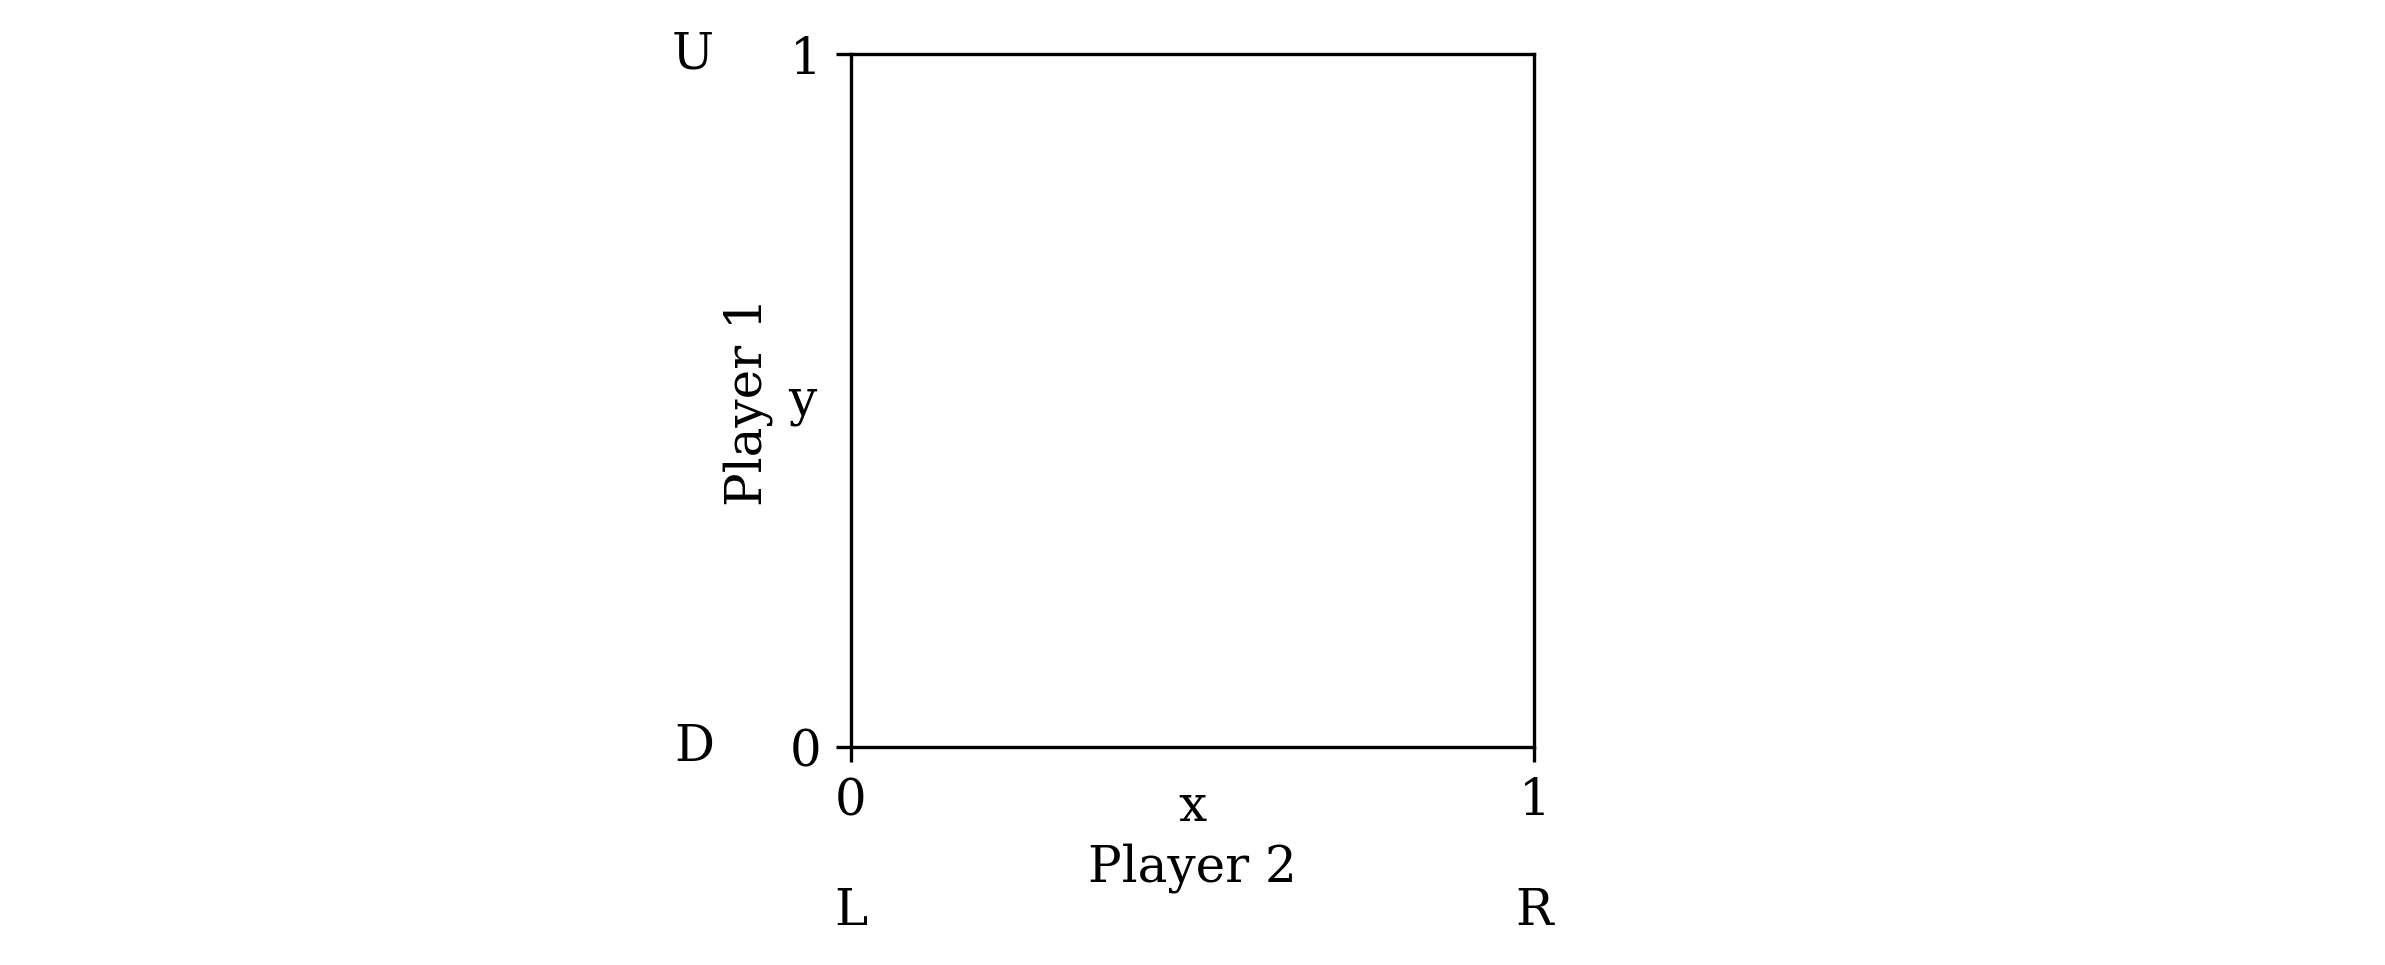
\includegraphics[width=\textwidth]{Images/mixed_strategy_graph.png}
\end{figure}

\begin{enumerate}[label=\alph*), start=5]
\item  List all dominant strategies for this game (\textit{if none, write "none"}). \hfill \raisebox{-1ex}{\rule{4.2cm}{1pt}}

\end{enumerate}
\begin{enumerate}[label=\alph*), start=6]
\item  What is the fitness of A when the population mix is all A? \hfill \raisebox{-1ex}{\rule{4.2cm}{1pt}}

\end{enumerate}
\begin{enumerate}[label=\alph*), start=7]
\item  What is the fitness of B when the population mix is all A? \hfill \raisebox{-1ex}{\rule{4.2cm}{1pt}}

\end{enumerate}
\begin{enumerate}[label=\alph*), start=8]
\item  Is A ESS? \hfill \raisebox{-1ex}{\rule{4.2cm}{1pt}}

\end{enumerate}
\begin{enumerate}[label=\alph*), start=9]
\item  What is the fitness of A when the population mix is all B? \hfill \raisebox{-1ex}{\rule{4.2cm}{1pt}}

\end{enumerate}
\begin{enumerate}[label=\alph*), start=10]
\item  What is the fitness of B when the population mix is all B? \hfill \raisebox{-1ex}{\rule{4.2cm}{1pt}}

\end{enumerate}
\begin{enumerate}[label=\alph*), start=11]
\item  Is B ESS? \hfill \raisebox{-1ex}{\rule{4.2cm}{1pt}}

\end{enumerate}
\begin{enumerate}[label=\alph*), start=12]
\item  Label all ESS and their values on the phase space graph below.
\end{enumerate}

\begin{figure}[h!]
\centering
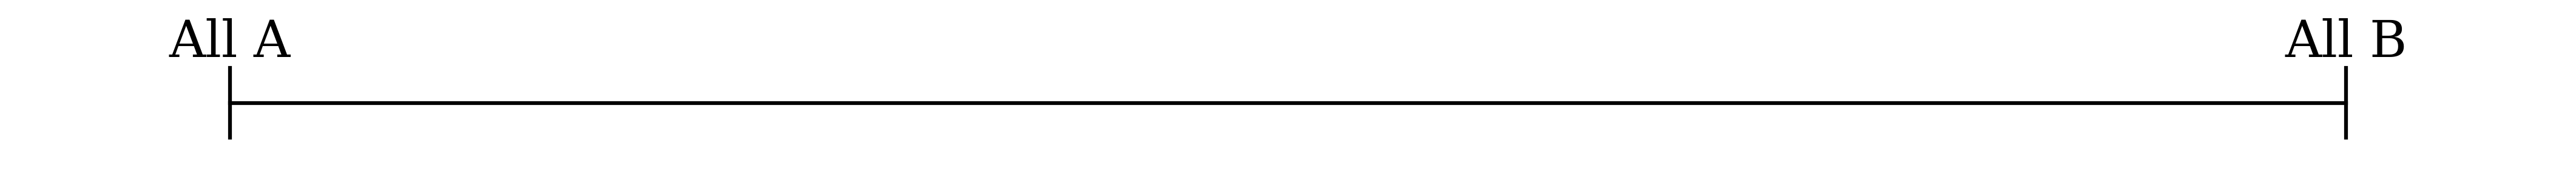
\includegraphics[width=\textwidth]{Images/phase_space_graph.png}
\end{figure}

\pagebreak

\subsection*{Game 3 (of 11). Use Version 1 for a through e. Use Version 2 for f through l.
}
$$
\begin{array}{lcr}
\begin{array}{lccc}
    & & & \textbf{Version 1} \\
    & & & (1-x) \ \ \ \ x\\
    & & & \text{L} \ \ \ \ \text{R}\\
    & &
    \begin{array}{r}
        y \ \ \text{U} \\
        (1-y) \ \ \text{D} \\
    \end{array} &
    \begin{array}{|c|c|}
        \hline
        12,12 & 5,12 \\
        \hline
        12,5 & 16,16 \\
        \hline
    \end{array}
\end{array}
&
\begin{array}{lccc}
    & & & \textbf{Version 2} \\
    & & & (1-f) \ \ \ \ f\\
    & & & \text{A} \ \ \ \ \text{B}\\
    & &
    \begin{array}{r}
        \text{A} \\
        \text{B} \\
    \end{array} &
    \begin{array}{|c|c|}
        \hline
        12 & 5 \\
        \hline
        12 & 16 \\
        \hline
    \end{array}
\end{array}
\end{array}
$$


\begin{enumerate}[label=\alph*), start=1]
\item  Which outcomes are Pareto optimal (\textit{if none, write "none"})? \hfill \raisebox{-1ex}{\rule{4.2cm}{1pt}}

\end{enumerate}
\begin{enumerate}[label=\alph*), start=2]
\item  List all NE in pure strategies. \hfill \raisebox{-1ex}{\rule{4.2cm}{1pt}}

\end{enumerate}
\begin{enumerate}[label=\alph*), start=3]
\item  Is this game zero sum? \hfill \raisebox{-1ex}{\rule{4.2cm}{1pt}}

\end{enumerate}
\begin{enumerate}[label=\alph*), start=4]
\item  Plot both player’s best responses and all MSNE on the graph below.

\end{enumerate}

\begin{figure}[h!]
\centering
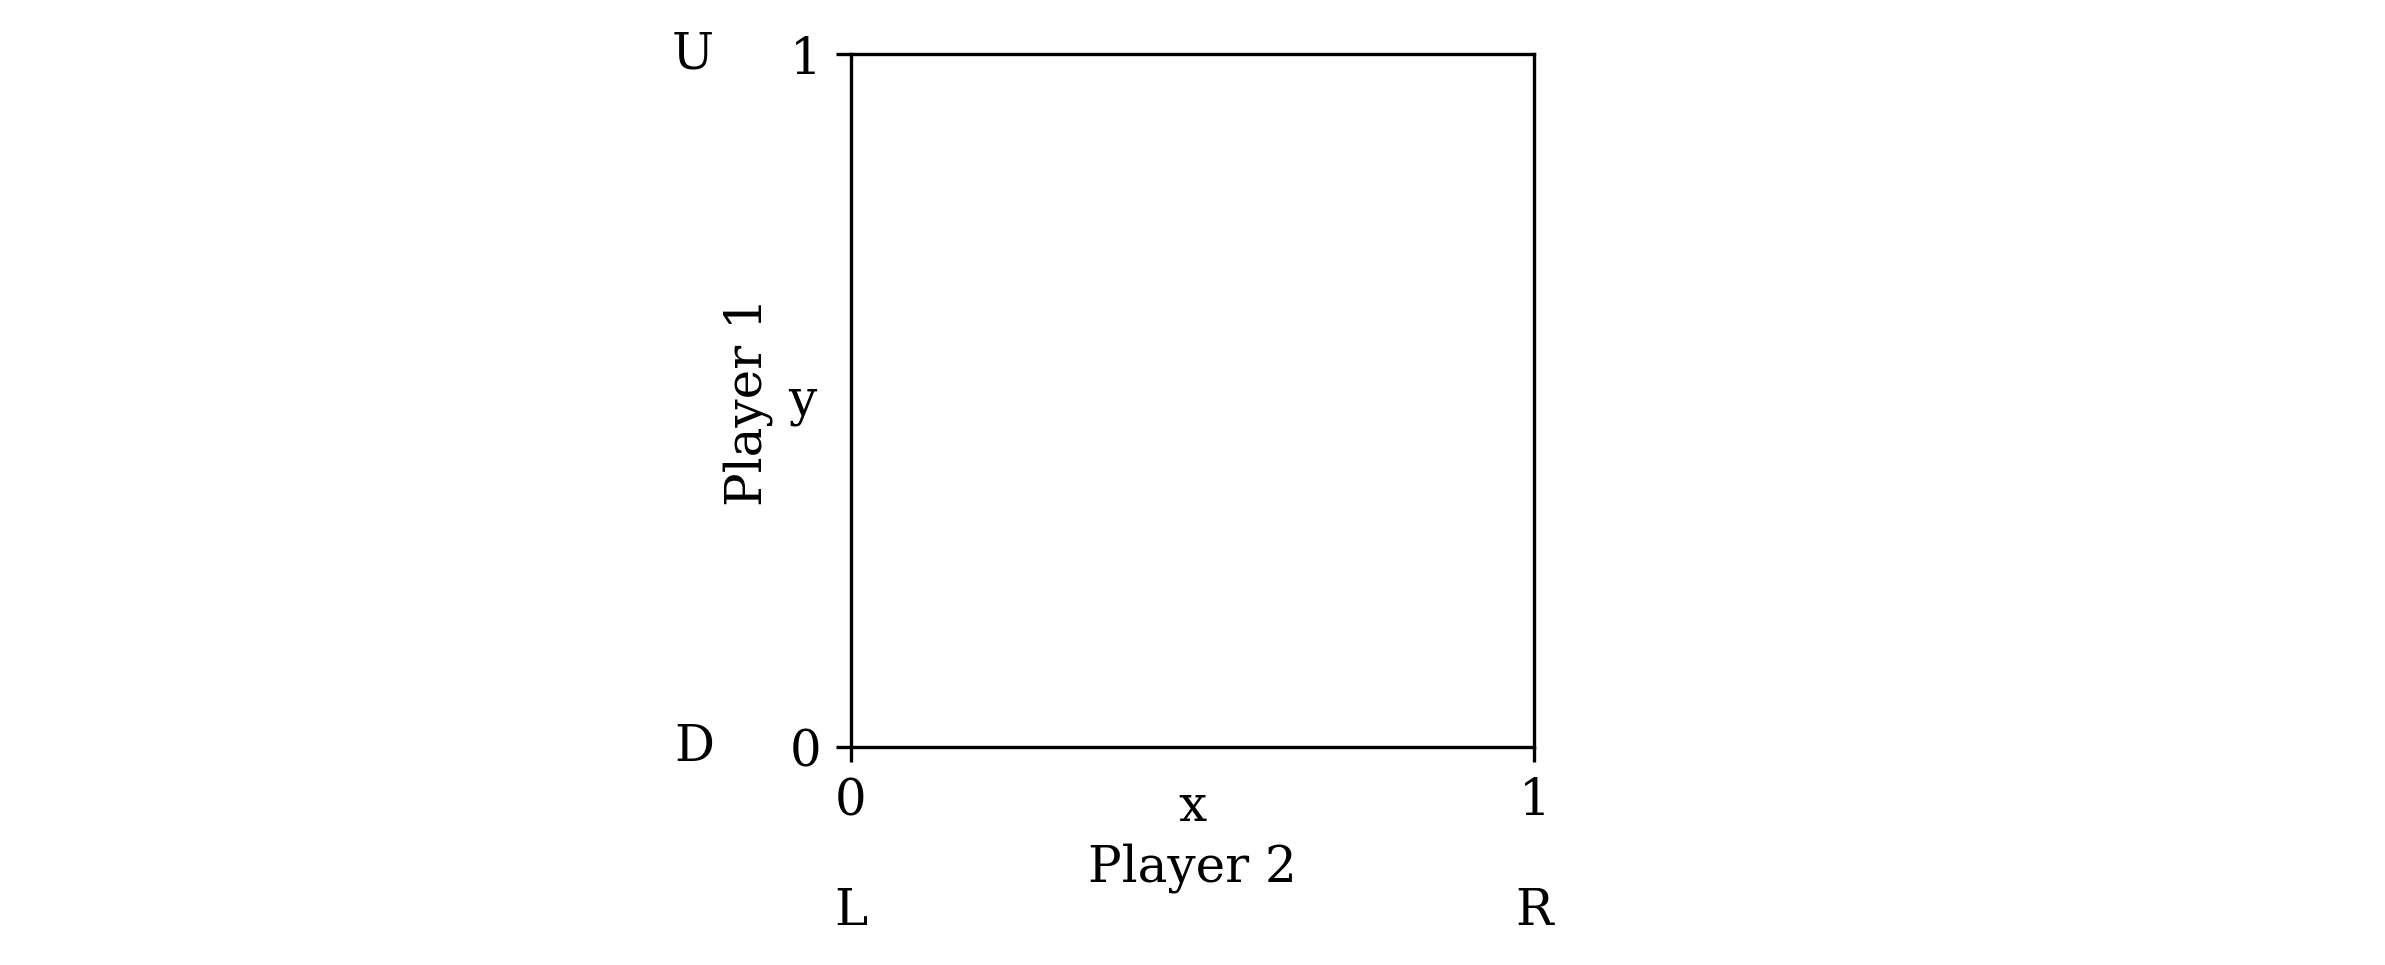
\includegraphics[width=\textwidth]{Images/mixed_strategy_graph.png}
\end{figure}

\begin{enumerate}[label=\alph*), start=5]
\item  List all dominant strategies for this game (\textit{if none, write "none"}). \hfill \raisebox{-1ex}{\rule{4.2cm}{1pt}}

\end{enumerate}
\begin{enumerate}[label=\alph*), start=6]
\item  What is the fitness of A when the population mix is all A? \hfill \raisebox{-1ex}{\rule{4.2cm}{1pt}}

\end{enumerate}
\begin{enumerate}[label=\alph*), start=7]
\item  What is the fitness of B when the population mix is all A? \hfill \raisebox{-1ex}{\rule{4.2cm}{1pt}}

\end{enumerate}
\begin{enumerate}[label=\alph*), start=8]
\item  Is A ESS? \hfill \raisebox{-1ex}{\rule{4.2cm}{1pt}}

\end{enumerate}
\begin{enumerate}[label=\alph*), start=9]
\item  What is the fitness of A when the population mix is all B? \hfill \raisebox{-1ex}{\rule{4.2cm}{1pt}}

\end{enumerate}
\begin{enumerate}[label=\alph*), start=10]
\item  What is the fitness of B when the population mix is all B? \hfill \raisebox{-1ex}{\rule{4.2cm}{1pt}}

\end{enumerate}
\begin{enumerate}[label=\alph*), start=11]
\item  Is B ESS? \hfill \raisebox{-1ex}{\rule{4.2cm}{1pt}}

\end{enumerate}
\begin{enumerate}[label=\alph*), start=12]
\item  Label all ESS and their values on the phase space graph below.
\end{enumerate}

\begin{figure}[h!]
\centering
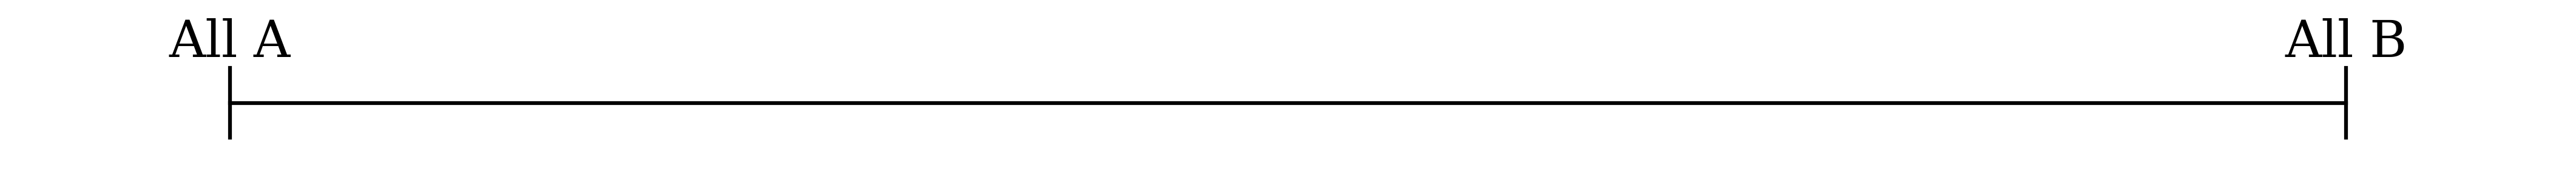
\includegraphics[width=\textwidth]{Images/phase_space_graph.png}
\end{figure}

\pagebreak

\subsection*{Game 4 (of 11). For the following game:
}
$$
\begin{array}{lccc}
    & & & \text{L} \ \ \ \ \text{R}\\
    & &
    \begin{array}{r}
        \text{U} \\
        \text{D} \\
    \end{array} &
    \begin{array}{|c|c|}
        \hline
        200,200 & 12,210 \\
        \hline
        210,12 & 50,50 \\
        \hline
    \end{array}
\end{array}
$$



\begin{enumerate}[label=\alph*), start=1]
\item  In an infinitely repeated setting, what is the present value of playing Grim-Trigger against Grim-Trigger?

\end{enumerate}
\hfill \raisebox{-1ex}{\rule{4.2cm}{1pt}}

\vspace{1cm}

\begin{enumerate}[label=\alph*), start=2]
\item  In an infinitely repeated setting, what is the present value of playing D in all periods against Grim-Trigger? \hfill \raisebox{-1ex}{\rule{4.2cm}{1pt}}

\end{enumerate}
\vspace{1cm}

\begin{enumerate}[label=\alph*), start=3]
\item  In an infinitely repeated setting, for what discount factors $\delta$ can cooperation be sustained against Grim-Trigger? \hfill \raisebox{-1ex}{\rule{4.2cm}{1pt}}

\end{enumerate}
\vspace{2cm}

\begin{enumerate}[label=\alph*), start=4]
\item  In an infinitely repeated setting, what is the present value of playing Tit-For-Tat against Tit-For-Tat? 

\end{enumerate}
\hfill \raisebox{-1ex}{\rule{4.2cm}{1pt}}

\vspace{1cm}

\begin{enumerate}[label=\alph*), start=5]
\item  In an infinitely repeated setting, what is the present value of playing D in the first period and Tit-For-Tat afterward against Tit-For-Tat?

\end{enumerate}
\hfill \raisebox{-1ex}{\rule{4.2cm}{1pt}}

\vspace{1cm}

\begin{enumerate}[label=\alph*), start=6]
\item  In an infinitely repeated setting, for what discount factors $\delta$ can cooperation be sustained against Tit-For-Tat? 

\end{enumerate}
\hfill \raisebox{-1ex}{\rule{4.2cm}{1pt}}

\vspace{2cm}

\begin{enumerate}[label=\alph*), start=7]
\item  In an indefinitely repeated game, if the probability of playing subsequent rounds is 7\% after each round concludes, which strategies sustain cooperation – Grim Trigger, Tit-for-tat, both, or neither? 

\end{enumerate}
\hfill \raisebox{-1ex}{\rule{4.2cm}{1pt}}


\pagebreak

\subsection*{Game 5 (of 11). For the following game:
}
$$
\begin{array}{lccc}
    & & & (1-f) \ \ \ \ f\\
    & & & \text{A} \ \ \ \ \text{B}\\
    & &
    \begin{array}{r}
        \text{A} \\
        \text{B} \\
    \end{array} &
    \begin{array}{|c|c|}
        \hline
        7,7 & 26,6 \\
        \hline
        6,26 & 19,19 \\
        \hline
    \end{array}
\end{array}
$$



\begin{enumerate}[label=\alph*), start=1]
\item  Which outcomes are Pareto optimal (\textit{if none, write "none"})? \hfill \raisebox{-1ex}{\rule{4.2cm}{1pt}}

\end{enumerate}
\begin{enumerate}[label=\alph*), start=2]
\item  List all NE in pure strategies \hfill \raisebox{-1ex}{\rule{4.2cm}{1pt}}

\end{enumerate}
\begin{enumerate}[label=\alph*), start=3]
\item  Is this game zero sum? \hfill \raisebox{-1ex}{\rule{4.2cm}{1pt}}

\end{enumerate}
\begin{enumerate}[label=\alph*), start=4]
\item  When starting from a population mix of 50-50, what is the population mix of A after 1 gen?

\end{enumerate}
\hfill \raisebox{-1ex}{\rule{4.2cm}{1pt}}

\vspace{2cm}

\begin{enumerate}[label=\alph*), start=5]
\item  Label all ESS and their values on the phase space graph below.

\end{enumerate}

\begin{figure}[h!]
\centering
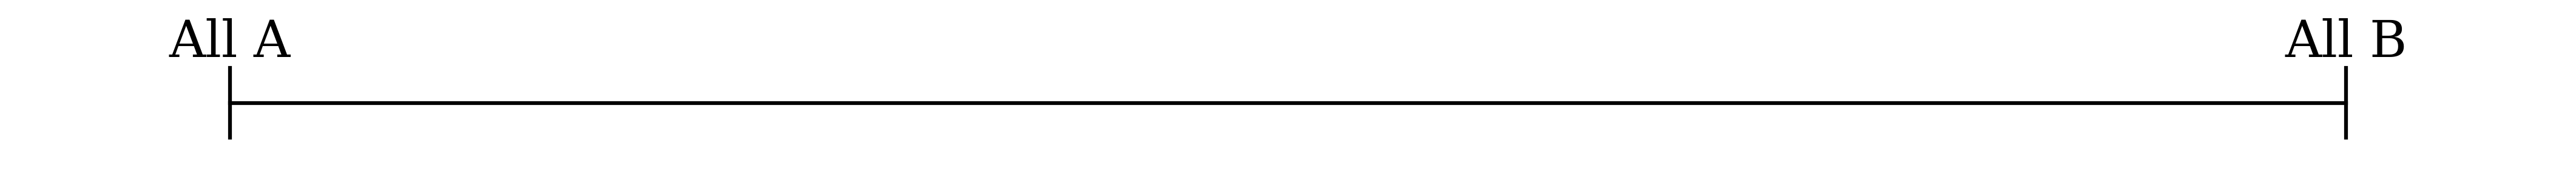
\includegraphics[width=\textwidth]{Images/phase_space_graph.png}
\end{figure}

\subsection*{Game 6 (of 11). For the following game:
}

\begin{enumerate}[label=\alph*), start=1]
\item  List all NE in pure strategies. \hfill \raisebox{-1ex}{\rule{4.2cm}{1pt}}

\end{enumerate}
\begin{enumerate}[label=\alph*), start=2]
\item  List all SPNE in pure strategies. \hfill \raisebox{-1ex}{\rule{4.2cm}{1pt}}

\end{enumerate}


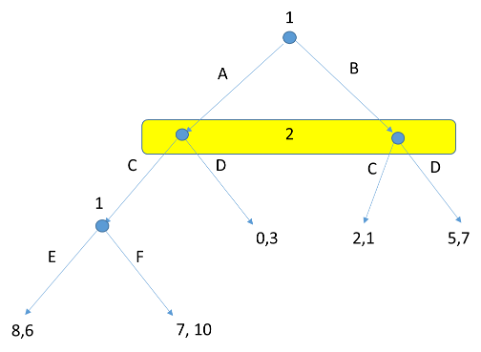
\includegraphics{Images/FinalGameTree1.png}


\pagebreak

\subsection*{Game 7 (of 11). For the following game:
}

\begin{enumerate}[label=\alph*), start=1]
\item  List all NE in pure strategies. \hfill \raisebox{-1ex}{\rule{4.2cm}{1pt}}

\end{enumerate}
\begin{enumerate}[label=\alph*), start=2]
\item  List all SPNE in pure strategies. \hfill \raisebox{-1ex}{\rule{4.2cm}{1pt}}

\end{enumerate}


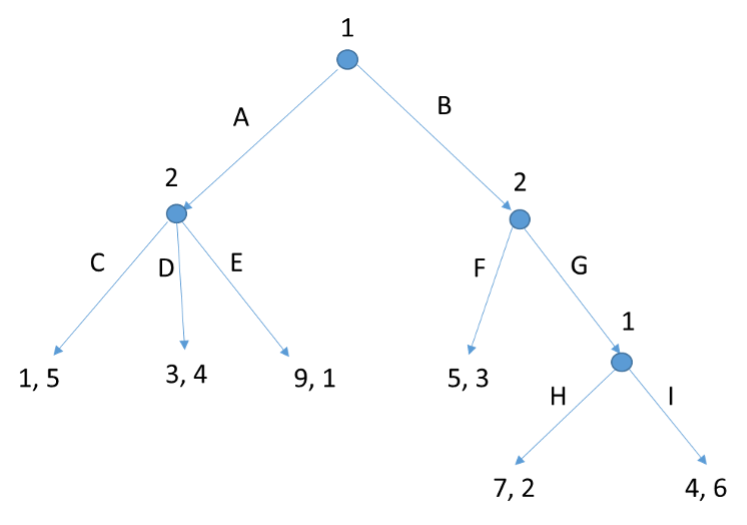
\includegraphics{Images/Picture7.png}


\pagebreak

\subsection*{Game 8 (of 11). Keynesian Beauty Contest 
}

Suppose a very large number of players are trying to guess a target number T, where the target is equal to 3/4 of the average plus 20.  

\begin{enumerate}[label=\alph*), start=1]
\item  Write the mathematical relationship between the Nash equilibrium guess and the Target. 

\end{enumerate}
\hfill \raisebox{-1ex}{\rule{4.2cm}{1pt}}

\begin{enumerate}[label=\alph*), start=2]
\item  Write the mathematical relationship between the Nash equilibrium guess and the average guess. 

\end{enumerate}
\hfill \raisebox{-1ex}{\rule{4.2cm}{1pt}}

\begin{enumerate}[label=\alph*), start=3]
\item  What is the Nash equilibrium? \hfill \raisebox{-1ex}{\rule{4.2cm}{1pt}}

\end{enumerate}

\subsection*{Game 9 (of 11). Symmetric Cournot Competition
}
Suppose there are 2 firms in an industry. Demand is represented by the following equation:  
$P = 710 - Q$. All firms are symmetric with a marginal cost of $50$. 

\begin{enumerate}[label=\alph*), start=1]
\item  What is firm 1’s profit function if there are 2 firms? \hfill \raisebox{-1ex}{\rule{4.2cm}{1pt}}

\end{enumerate}
\vspace{1cm}

\begin{enumerate}[label=\alph*), start=2]
\item  What is the best response function for firm 1 if there are 2 firms? \hfill \raisebox{-1ex}{\rule{4.2cm}{1pt}}

\end{enumerate}
\vspace{1cm}

\begin{enumerate}[label=\alph*), start=3]
\item  What is the equilibrium quantity and price for firm 1 with 2 firms? \hfill \raisebox{-1ex}{\rule{4.2cm}{1pt}}

\end{enumerate}
\vspace{1cm}

\begin{enumerate}[label=\alph*), start=4]
\item  If there were 3 firms, what is firm 1’s equilibrium quantity and price? \hfill \raisebox{-1ex}{\rule{4.2cm}{1pt}}

\end{enumerate}

\pagebreak

\subsection*{Game 10 (of 11). Ultimatum Game
}
Consider an Ultimatum game with counter-offers that can only be split by $\$1$. The initial pool is $\$105$ and declines by $\$25$ with each counter offer and has a minimum of $\$0$. Players will only accept an offer if it is better than what they can make by counter-offering. Players are “rational” and have full (common) knowledge relating to the game. What is the SPNE initial offer? \hfill \raisebox{-1ex}{\rule{4.2cm}{1pt}}

\vspace{6cm}


\subsection*{Game 11 (of 11). Vote Counting
}
20 voters prefer: A > B > C > D

10 voters prefer: B > A > D > C

8 voters prefer: B > D > C > A

7 voters prefer: D > B > C > A

4 voters prefer: C > B > D > A

\begin{enumerate}[label=\alph*), start=1]
\item  Which alternative wins a Plurality vote? \hfill \raisebox{-1ex}{\rule{4.2cm}{1pt}}

\end{enumerate}
\vspace{1cm}

\begin{enumerate}[label=\alph*), start=2]
\item  Does Plurality voting select the Condorcet Winner? \hfill \raisebox{-1ex}{\rule{4.2cm}{1pt}}

\end{enumerate}
\vspace{1cm}

\begin{enumerate}[label=\alph*), start=3]
\item  Which alternative wins using a Borda Count (\textit{3 points for 1st, 2 points for 2nd,...}) to pick the top two, then an Instant Runoff using the top two? \hfill \raisebox{-1ex}{\rule{4.2cm}{1pt}}

\end{enumerate}



\end{document}